\documentclass[compress]{beamer}
\usepackage{xcolor}
\usepackage{geometry}
\usepackage{setspace}
\usepackage{amsmath,amsfonts,amssymb,amsthm}
\usepackage{graphicx}
\usepackage{hyperref}
\usepackage[ruled,vlined]{algorithm2e}

\definecolor{SectionBackground}{HTML}{6A6AEC}
\definecolor{SectionName}{HTML}{0000FF}
\definecolor{Background}{HTML}{D9D9D9}

\setbeamercolor{sidebar}{bg=Background}
\setbeamercolor{section in sidebar shaded}{fg=SectionName}
\setbeamercolor{background canvas}{bg=white}
\setbeamercolor{section in toc}{fg=SectionName}
\setbeamercolor{palette sidebar secondary}{fg=SectionName,bg=SectionBackground}

\useoutertheme[width=2cm,right]{sidebar}
\setbeamercolor{frametitle}{bg=white,fg=SectionName}
\setbeamercolor{logo}{bg=Background}

\setbeamercolor{block title}{bg=blue!15,fg=blue}
\setbeamercolor{block body}{bg=blue!5}

\setbeamertemplate{bibliography item}{\insertbiblabel}

\title{Community Structure Identification}
\logo{
\includegraphics[width=1.5cm]{Pics/Logo/hcmut.png}}

% \AtBeginSection[]{
%     \begin{frame}
%         \frametitle{Overview}
%         \tableofcontents[currentsection]
%     \end{frame}
% }

\begin{document}

\begin{frame}[t]  
    \Large Maths Foundation for Computer Science \\
    \textcolor{SectionName}{ Community Structure Identification}

    \normalsize
    \vspace{1.5cm}
    
    \begin{table}[h]
        \begin{tabular}{rrl}
            \hspace{1.5cm}
            & \textbf{Lecturer:} 
            & Nguyen An Khuong, Ph.D \\
            && Tran Tuan Anh, Ph.D \\
            & \textbf{Students:} 
            & Ha Trung Kien	- 2013540 \\
            & & Nguyen Huy Hoang - 2013230 \\
            & & Do Minh Tam - 2470093 \\
            & & Nguyen Trong Phuc - 2470289 \\
            & & Lam Hoang Tan - 2213054 \\
            & & Tran Nhu Mai Anh - 2210140 \\
        \end{tabular}
    \end{table}
\end{frame}

\begin{frame}{Contents}
    \tableofcontents
\end{frame}

\section{Introduction}

\begin{frame}[t]{Motivation}
    \begin{itemize}
        \item Graph Theory: Fundamental in mathematics and computer science, modeling complex relationships for solving real-world problems.
        \item Social Networks: Growth has led to studying online communities using graphs.
        \item Community Detection:
        \begin{itemize}
            \item \textit{Hierarchical Clustering}: Groups nodes in tree-like structures for multi-level relationships.
            \item \textit{Girvan-Newman Algorithm}: Identifies clusters by iterative edge removal based on betweenness.
            \item \textit{Louvain Algorithm}: Optimizes modularity for efficient detection of cohesive groups.
        \end{itemize}
        \item Applications: Insights into social behavior, marketing, sociology, and network management.
    \end{itemize}
\end{frame}

\begin{frame}[t]{Problem}
    \begin{itemize}
        \item Objective: Build a book recommendation system based on customer co-purchasing behavior.
        \item Dataset: Political Books Dataset.
        \begin{itemize}
            \item 105 book IDs, 441 co-purchase relationships.
            \item Nodes: Books, Edges: Co-purchased books.
            \item File \textit{out.dimacs10-polbooks}, each line representing co-purchased book pairs.
        \end{itemize}
        \item Problem:
        \begin{itemize}
            \item Perform clustering to identify communities of frequently co-purchased books.
            \item Visualize the graph representation of these communities.
        \end{itemize}
    \end{itemize}
\end{frame}

\section{Preliminaries}

\begin{frame}[t]{Graph Concepts}
    \textbf{Types of graphs}

    \begin{itemize}
        \item Based on Directionality:
        \begin{itemize}
            \item Undirected Graphs
            \item Directed Graphs
        \end{itemize}

        \item Based on Weight:
        \begin{itemize}
            \item Weighted Graphs
            \item Unweighted Graphs
        \end{itemize}
        
        \item Special Graphs:
        \begin{itemize}
            \item Bipartite Graphs
            \item Complete Graphs
            \item Tree
        \end{itemize}

    \end{itemize}
\end{frame}

\begin{frame}[t]{Representations of a graph}
    \begin{figure}[H]
        \centering
        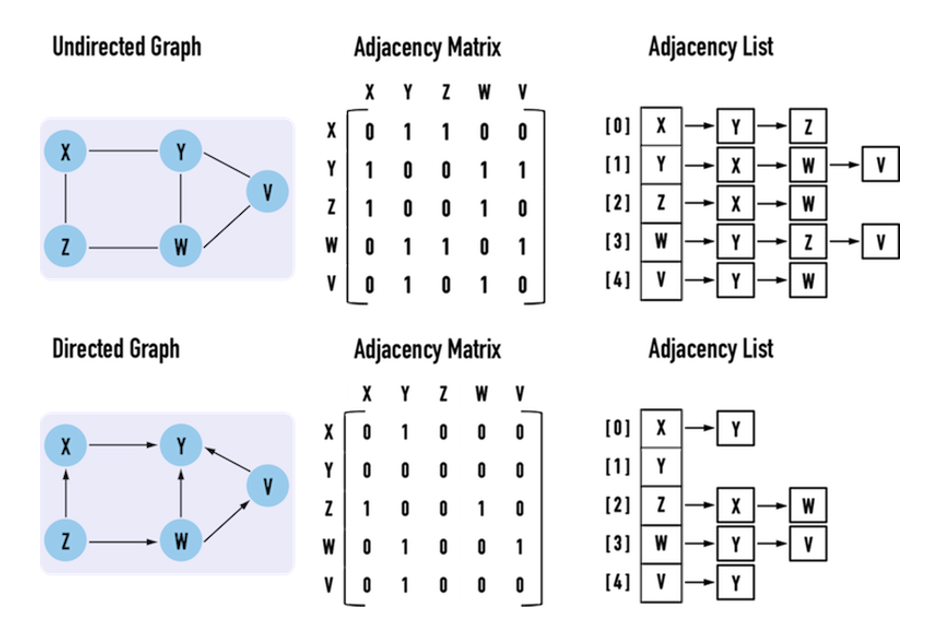
\includegraphics[width=8cm]{Pics/Adjacency_matrix_list.png}
        \caption{Example of an Adjacency Matrix and Adjacency List}
        \label{fig:girvan_example}
    \end{figure}
\end{frame}

\begin{frame}[t]{Social Network Communities}
    \begin{figure}[H]
        \centering
        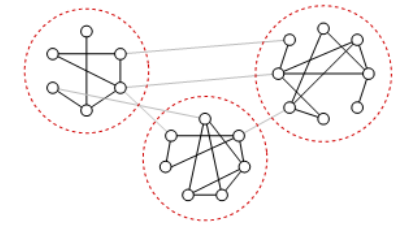
\includegraphics[width=6cm]{Pics/simple_social_network.png}
        \caption{A simple social network with three communities}
        \label{fig:girvan_example}
    \end{figure}
\end{frame}

\begin{frame}[t]{Community Detection Problems}
    \begin{block}{Introduction}
        \textit{Problem}: Detect communities in a social network and provide a list of nodes belonging to each community.

        \textit{Input}: A social network graph \(G = (V, E)\), where:
        \begin{itemize}
            \item \(V\) is the set of nodes: \(v_1, v_2, ..., v_n\)
            \item \(E\) is the set of edges: \(E = \{(v_i, v_j)\}\)
        \end{itemize}
        
        \textit{Output}: A set of communities \(C_i\) and the corresponding sets of nodes belonging to each community: \(\{C_1, C_2, ..., C_n\}\)
    \end{block}
\end{frame}

\begin{frame}[t]{Community Detection Problems}
    \begin{block}{Modularity}
        \begin{itemize}
            \item Modularity is a key metric in network analysis used to measure the quality of a community division in a graph.
            \item Modularity measures the fraction of edges that fall within communities minus the expected fraction of such edges if they were distributed randomly.
            \item A higher modularity score indicates better-defined community structures.
        \end{itemize}
    \end{block}
\end{frame}

\begin{frame}[t]{Community Detection Problems}
    \begin{block}{Modularity}
        For a graph \(G = (V, E)\) divided into communities, the modularity \(Q\) is given by:

        \[Q = \frac{1}{2m} \sum_{i,j} \left[ A_{ij} - \frac{k_i k_j}{2m} \right] \delta(c_i, c_j)\]
    \end{block}

    \begin{itemize}
        \item \(A_{ij}\): Adjacency matrix entry (1 if there's an edge between nodes \textit{i} and \textit{j}, 0 otherwise).
        \item \(k_i,k_j\): Degrees of nodes \textit{i} and \textit{j}
        \item \(m\): Total number of edges in the graph.
        \item \(\delta(c_i, c_j)\): the Kronecker delta (1 if nodes \textit{i} and \textit{j} are in the same community, 0 otherwise).
    \end{itemize}
\end{frame}

\begin{frame}[t]{Community Detection Problems}
    \begin{block}{Community-Based Modularity Formula}
        \[Q = \sum_{c=1}^{n_c} \left( \frac{l_c}{m} - \left( \frac{d_c}{2m} \right)^2 \right)\]
    \end{block}

    \begin{itemize}
        \item \(n_c\): Number of communities in the network.
        \item \(l_c\): Total number of edges within community \(c\).
        \item \(m\): Total number of edges in the graph.
        \item \(d_c\): Total degree (sum of node degrees) of all nodes in community \(c\).
    \end{itemize}
\end{frame}

\begin{frame}[t]{Modularity}
    \textbf{Example of Modularity Calculation}
    \begin{figure}[H]
        \begin{center}
        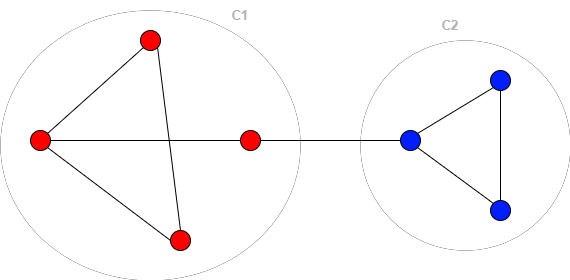
\includegraphics[width=5cm]{Pics/modularity_ex.png}   
        \end{center}
        \label{}
    \end{figure}
    \begin{align*}
        Q &= \sum_{c=1}^{n_c} \left( \frac{l_c}{m} - \left( \frac{d_c}{2m} \right)^2 \right) \\
        &= \left( \frac{l_{C_1}}{m} - \left( \frac{d_{C_1}}{2m} \right)^2 \right) + \left( \frac{l_{C_2}}{m} - \left( \frac{d_{C_2}}{2m} \right)^2 \right) \\
        &= \left( \frac{4}{8} - \left( \frac{9}{2 . 8} \right)^2 \right) + \left( \frac{3}{8} - \left( \frac{7}{2 . 8} \right)^2 \right) = 0.367
    \end{align*}

\end{frame}

\begin{frame}[t]{Modularity}
    \begin{block}{Interpretation}
        \begin{enumerate}
            \item \textit{Range}: Modularity values range from \(-0.5\) to \(1\), where
            \begin{itemize}
                \item A value close to 1 indicates strong community structure.
                \item A value close to 0 suggests no community structure.
                \item Negative values indicate that the division is worse than random.
            \end{itemize}
        
            \item \textit{Community Structure Quality}
            \begin{itemize}
                \item High Modularity: Many edges within communities, few between them.
                \item Low Modularity: Communities are poorly defined or overlap significantly.
            \end{itemize}
        \end{enumerate}
    \end{block}
\end{frame}

\begin{frame}[t]{Community Detection Problems}
    \begin{block}{Centrality}
        Centrality is a key concept in network analysis that measures the importance or influence of a node within a network. It helps identify nodes that play crucial roles in the overall structure of the network.
        \begin{itemize}
            \item Degree Centrality
            \item Betweenness Centrality
            \item Closeness Centrality
        \end{itemize}
    \end{block}
\end{frame}

\begin{frame}[t]{Centrality}
    \begin{block}{Degree Centrality}
        \begin{itemize}
            \item \textit{Definition}: Measures the number of direct connections a node has. A node with a high degree centrality is directly connected to many other nodes.
            \item \textit{Formula}:
        
            \[C_{D}(v) = k_v\]
        
            where \(k_v\) is the degree of node \(v\) (the number of edges incident to \(v\)).
        \end{itemize}
    \end{block}
\end{frame}

\begin{frame}[t]{Centrality}
    \begin{block}{Betweenness Centrality}
        \begin{itemize}
            \item \textit{Definition}:  Measures how often a node acts as a bridge along the shortest path between two other nodes. Nodes with high betweenness centrality control the flow of information across the network.
            \item \textit{Formula}:
        
            \[C_B(v) = \sum_{s,t \in V} \frac{\sigma_{st}(v)}{\sigma_{st}}\]
        
            where \(\sigma_{st}(v)\) is the total number of shortest paths from node \(s\) to \(t\), and \(\sigma_{st}(v)\) is the number of those paths that pass through node \(v\).
        \end{itemize}
    \end{block}
\end{frame}

\begin{frame}[t]{Centrality}
    \begin{block}{Closeness Centrality}
        \begin{itemize}
            \item \textit{Definition}:  Measures how close a node is to all other nodes in the network. A node with high closeness centrality can quickly interact with all other nodes.
            \item \textit{Formula}:
        
            \[C_C(v) = \frac{1}{\sum_{u \in V} d(v, u)}\]
        
            where \(d(v,u)\) is the shortest path distance between node \(v\) to \(u\).
        \end{itemize}
    \end{block}
\end{frame}

\section{Approaches}

%Hierarchical Clustering

\subsection{Hierarchical Clustering}
\begin{frame}[t]{Hierarchical Clustering Algorithm Overview}
Hierarchical Clustering is an algorithm that groups data into a tree of nested clusters. \\
    \textbf{Key Points:}
    \begin{itemize}
        \item Results are presented in a \textbf{dendrogram diagram}.
        \item The main types are: \textbf{Agglomerative (Bottom-up)} and \textbf{Divisive (Top-down)}.
    \end{itemize}
     
\end{frame}

\begin{frame}[t]{Hierarchical Clustering Algorithm Overview}
    \begin{figure}[H]
        \centering
        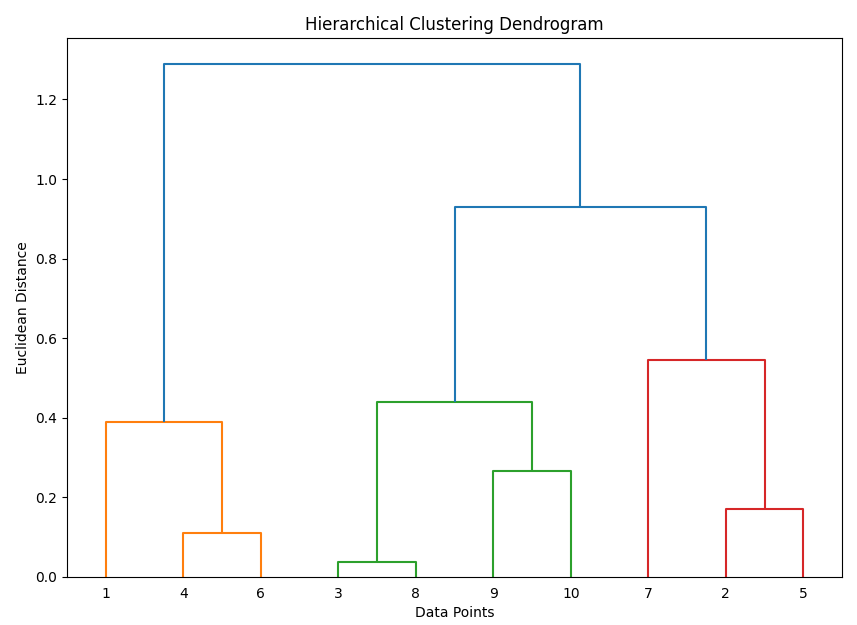
\includegraphics[width=230pt]{Pics/hierarchical/dendro.png}
        \caption{Hierarchical Clustering Dendrogram}
    \end{figure}
\end{frame}

\begin{frame}[t]{Hierarchical Clustering Algorithm Overview}
    \textbf{Mechanisms}
\begin{itemize}
    \item \textbf{Agglomerative (Bottom-up):} Starts with each object as an individual cluster and successively merges them into larger clusters.
    \item \textbf{Divisive (Top-down):} Starts with all objects in a single cluster and successively splits them into smaller clusters.
\end{itemize}
  \begin{figure}[H]
        \centering
        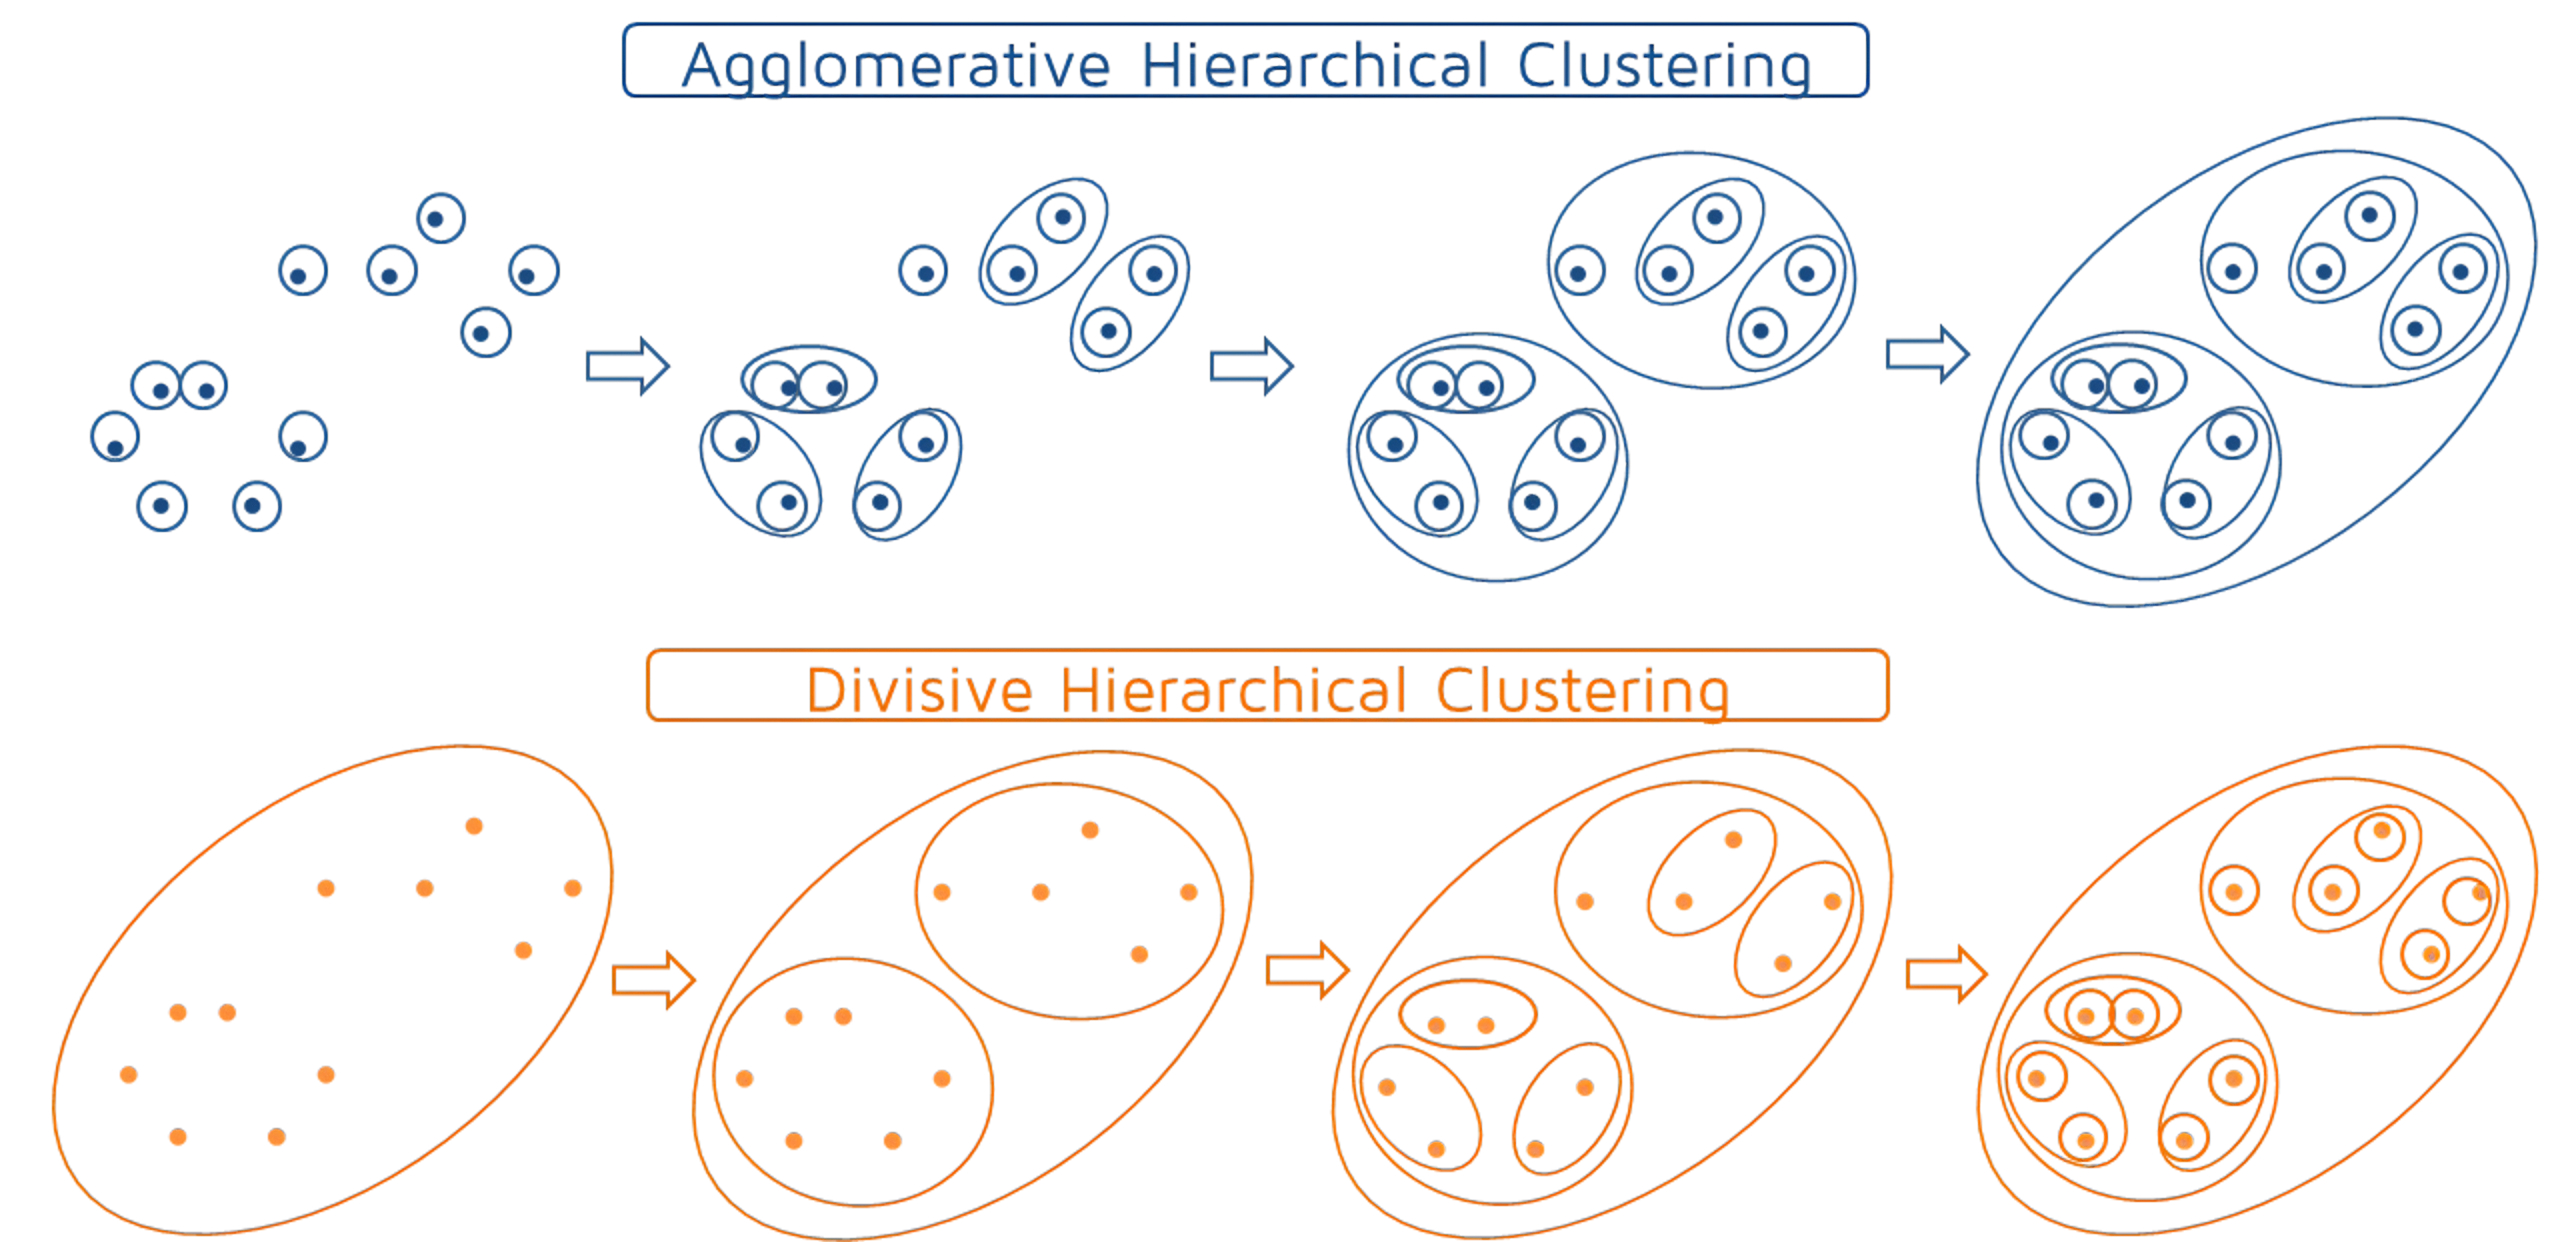
\includegraphics[width=200pt]{Pics/hierarchical/hierar_cluster.jpg}
        % \caption{Hierarchical Clustering Dendrogram}
    \end{figure}
\end{frame}

\begin{frame}[t]{Example of Agglomerative}
  \begin{figure}[H]
        \centering
        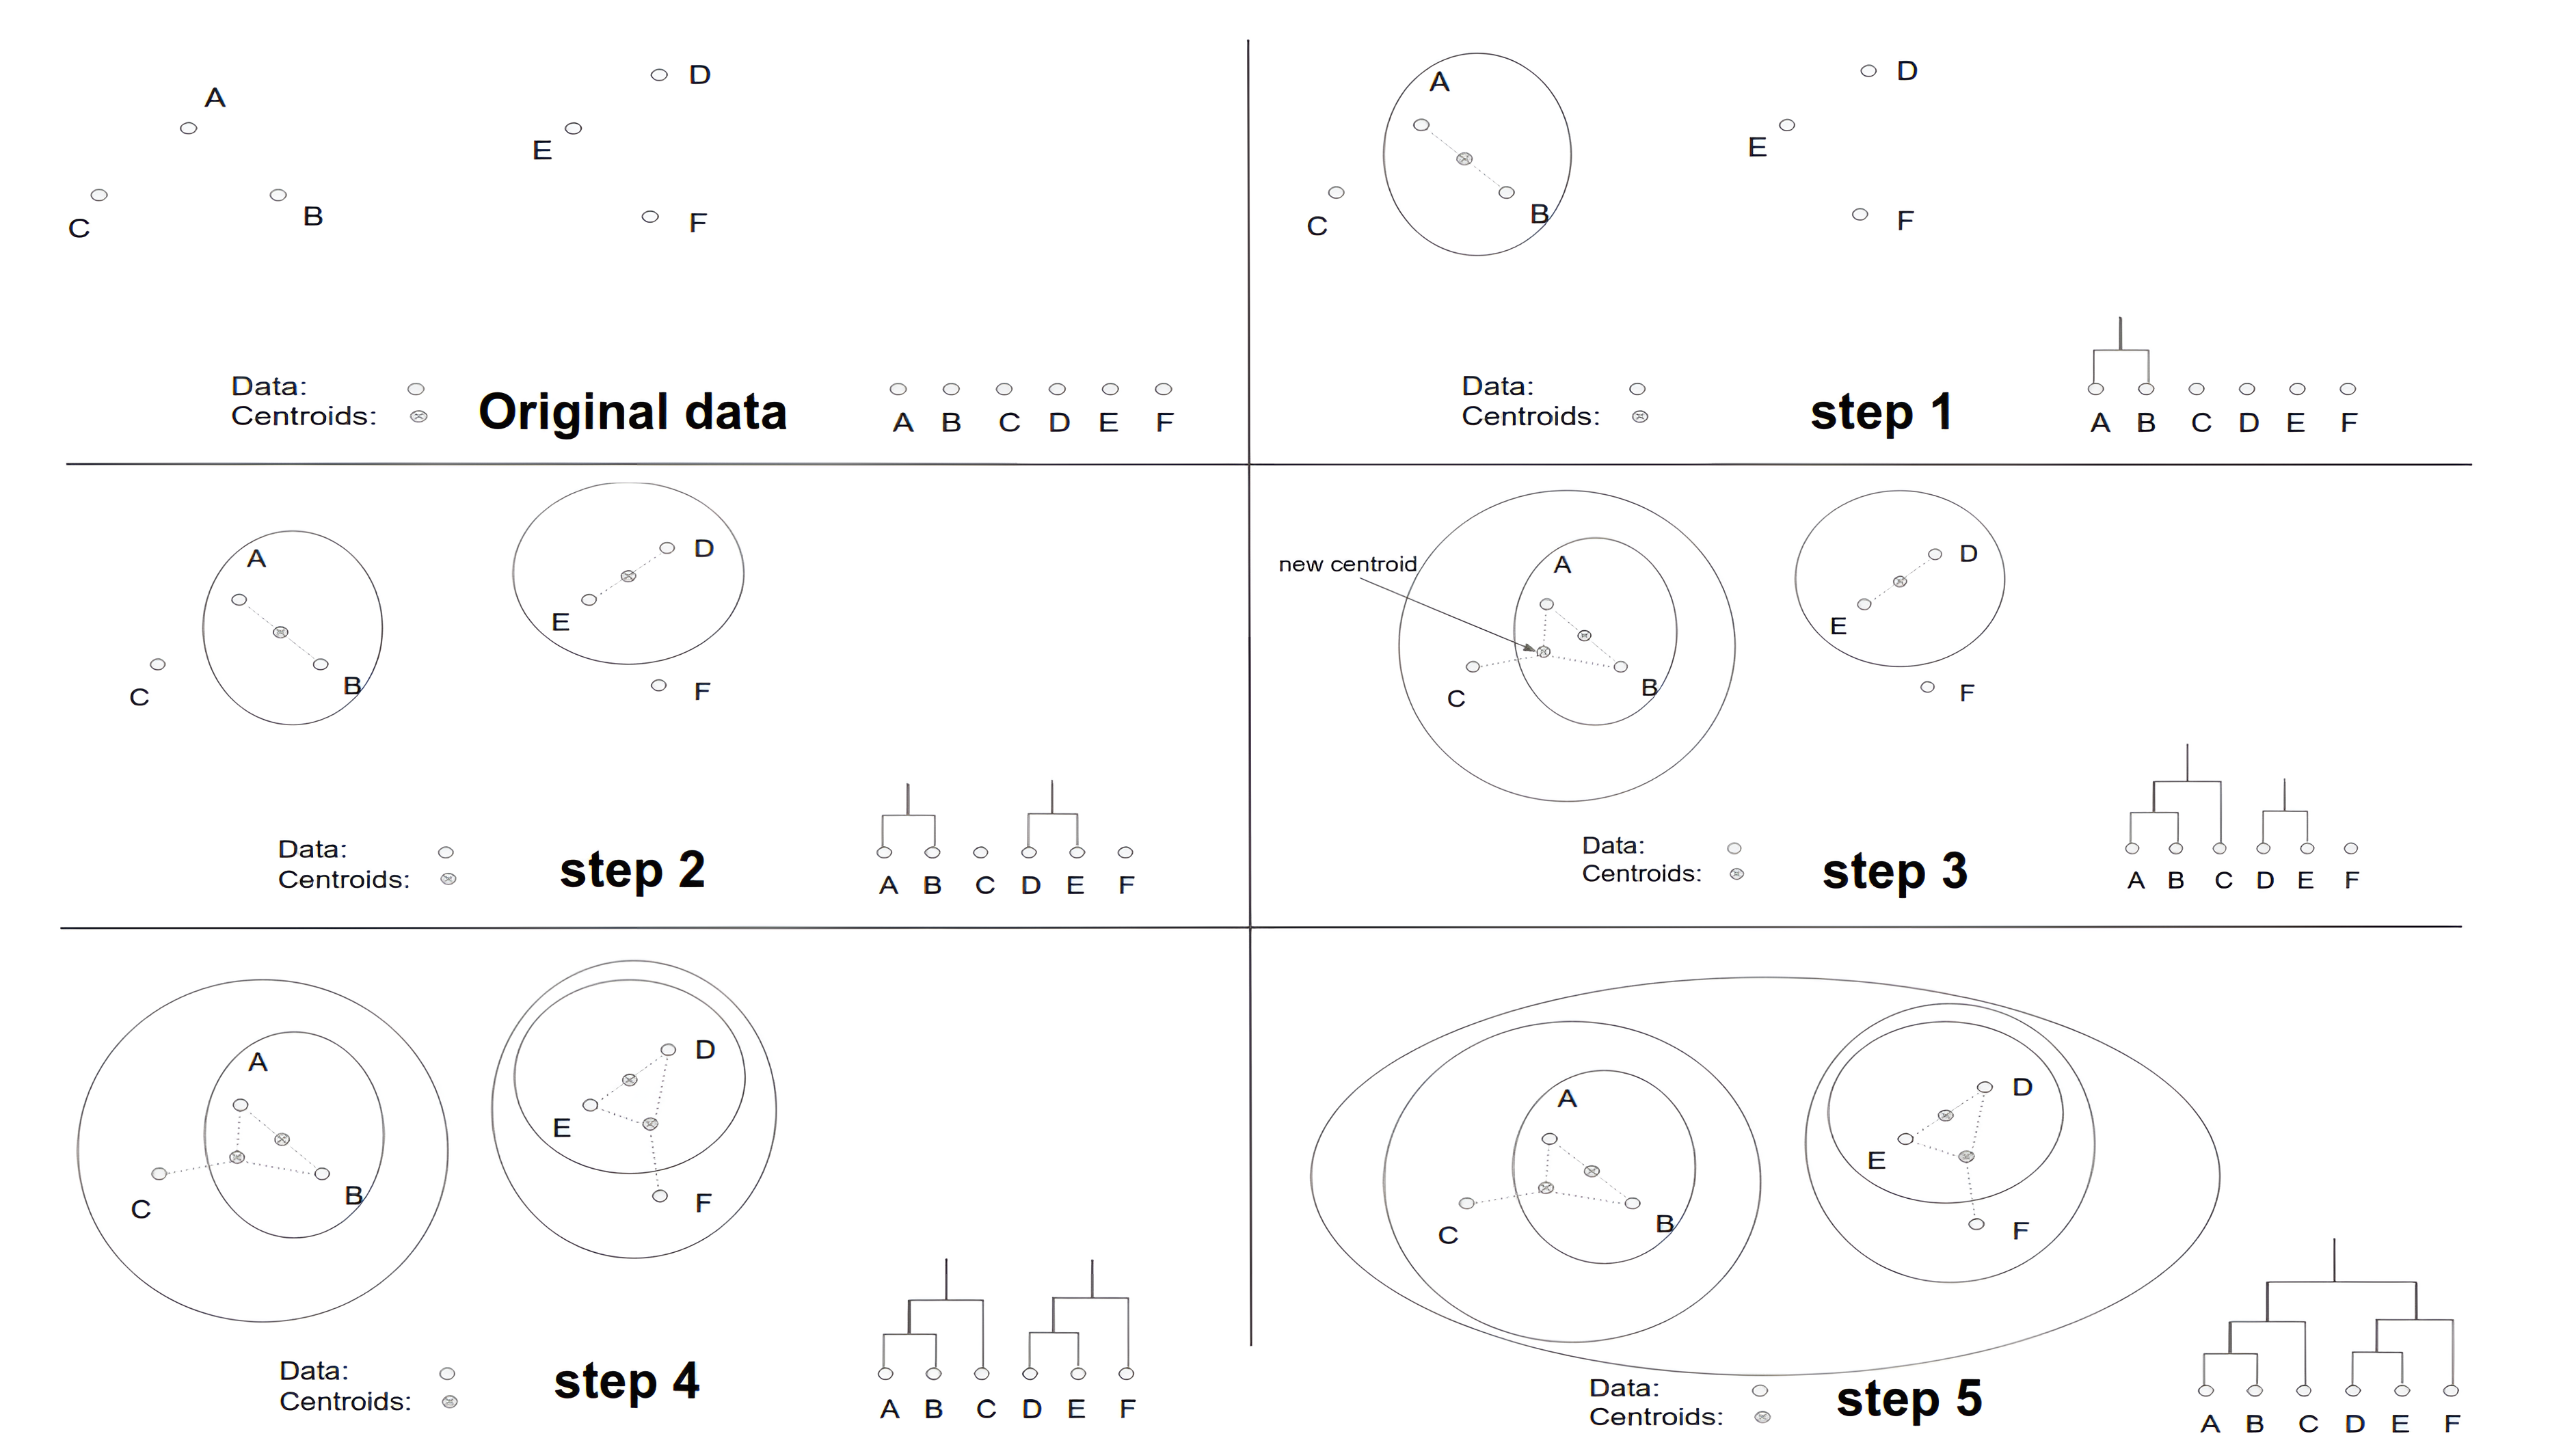
\includegraphics[width=285]{Pics/hierarchical/agg_e.png}
    \end{figure}
\end{frame}
\begin{frame}[t]{Example of Divisive}
  \begin{figure}[H]
        \centering
        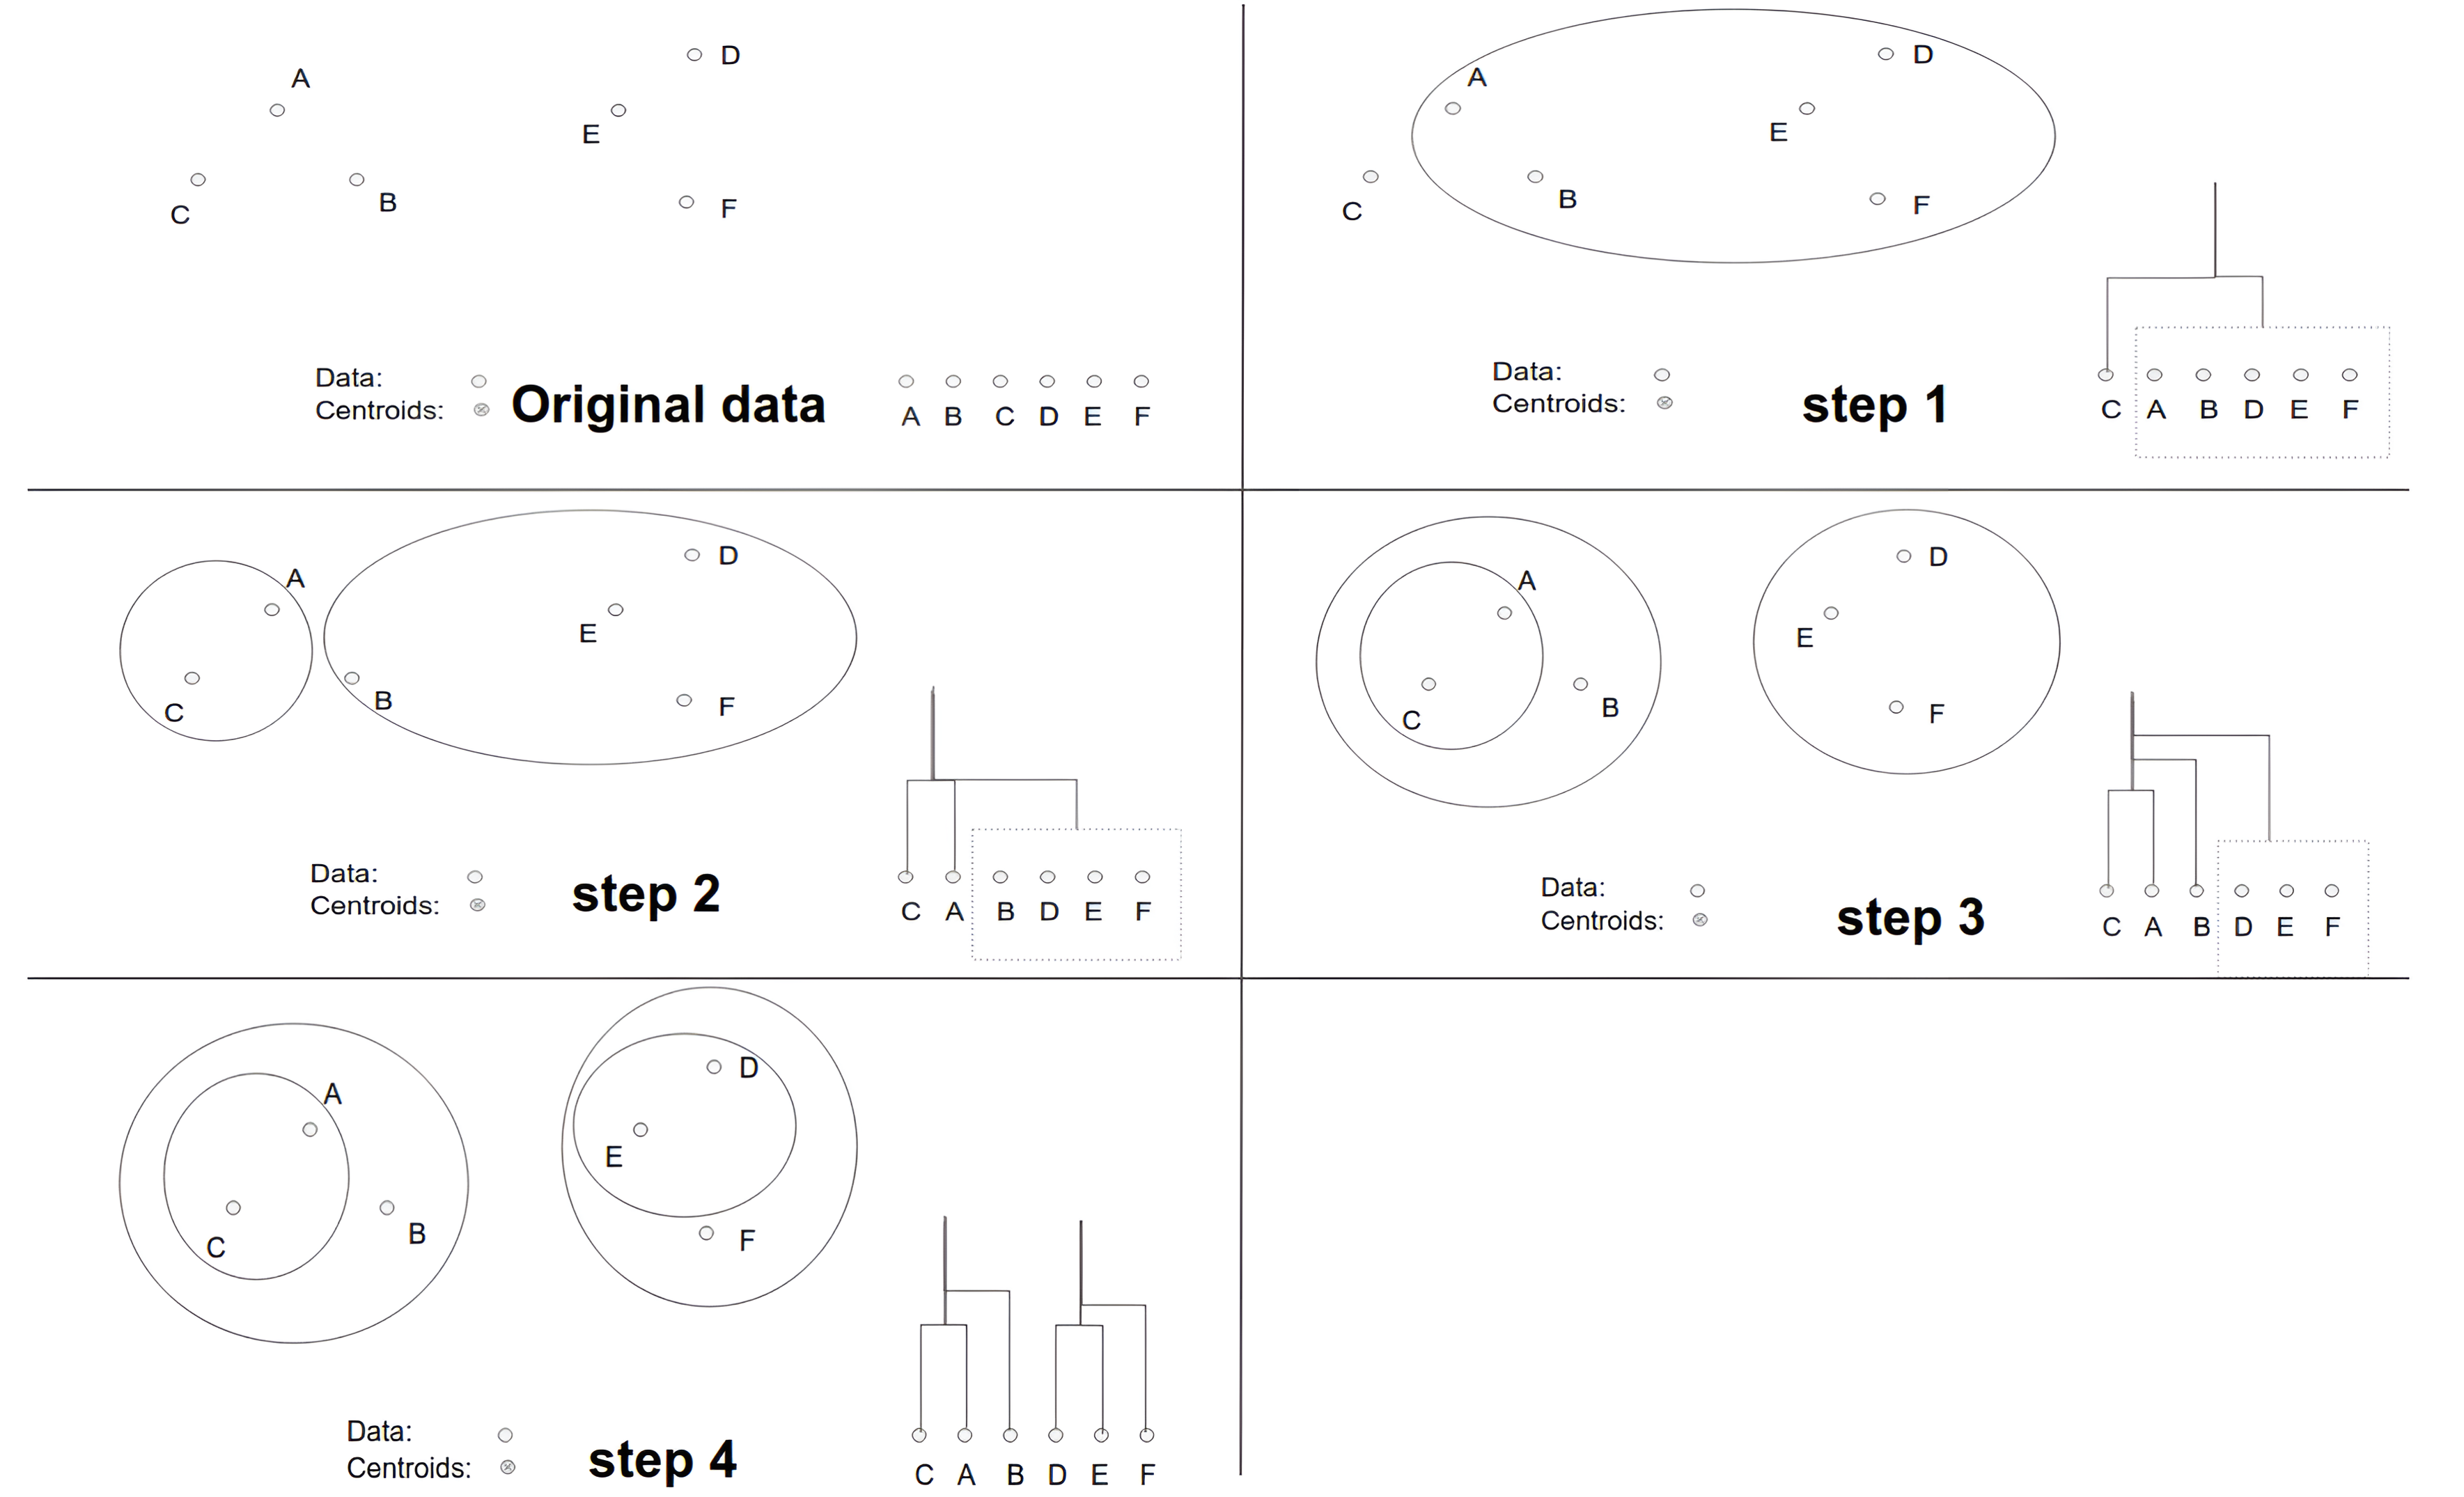
\includegraphics[width=285]{Pics/hierarchical/div_e.png}
    \end{figure}
\end{frame}

\begin{frame}[t]{Common Distance Metrics}
Suppose that $\mathcal{S}_1 = \{ \mathbf{x}_i^{(1)}\}_{i=1}^{N_1}$, and $\mathcal{S}_2 = \{ \mathbf{x}_j^{(2)} \}_{j=1}^{N_2}$ are two intermediary clusters that do not overlap.
\begin{itemize}
    \item \textbf{Single Linkage:} Minimum distance between points in two clusters.
\begin{equation}
d(\mathcal{S}_1, \mathcal{S}_2) = \min_{\mathbf{x}_i \in \mathcal{S}_1, \mathbf{x}_j \in \mathcal{S}_2} d(\mathbf{x}_i^{(1)}, \mathbf{x}_j^{(2)})
\end{equation}

    \item \textbf{Complete Linkage:} Maximum distance between points in two clusters.
\begin{equation}
d(\mathcal{S}_1, \mathcal{S}_2) = \max_{\mathbf{x}_i \in \mathcal{S}_1, \mathbf{x}_j \in \mathcal{S}_2} d(\mathbf{x}_i^{(1)}, \mathbf{x}_j^{(2)})
\end{equation}  

\item  \textbf{Average Linkage:} Mean distance between points in two clusters.
\begin{equation}
d(\mathcal{S}_1, \mathcal{S}_2) = \frac{1}{N_1 N_2}\sum_{i=1}^{N_1} \sum_{j=1}^{N_2} d(\mathbf{x}_i^{(1)}, \mathbf{x}_j^{(2)})
\end{equation}
\end{itemize}
\end{frame}

\begin{frame}[t]{Common Distance Metrics}
\begin{itemize}
\item  \textbf{Ward's Method:} Minimizes variance within clusters. Let’s first start with the Euclidean distance equation for the two centroids of the clusters:
\begin{equation}
d(\mathbf{m}_1,\mathbf{m}_2) = d(\mathbf{m}_2,\mathbf{m}_1) = \sqrt{\sum_{i=1}^{n} (m_i^{(1)}-m_i^{(2)})^2}
\end{equation}
Where $\mathbf{m}$, $\mathbf{m}_1$, and $\mathbf{m}_2$ are the centroids of $\mathcal{S}_1 \cup \mathcal{S}_2$, $\mathcal{S}_1$, and $\mathcal{S}_2$, respectively.

\end{itemize}
\end{frame}

\begin{frame}[t]{Common Distance Metrics}

Now the Ward linkage is given by this formula:
\begin{equation} \label{ward_linkage_1}
\begin{aligned}
d(\mathcal{S}_1, \mathcal{S}_2) & = \sum_{\mathbf{x}_i \in \mathcal{S_1} \cup \mathcal{S}_2} \| \mathbf{x}_i-\mathbf{m} \|^2 \\
& \quad - \sum_{\mathbf{x}_i \in \mathcal{S}_1} \| \mathbf{x}_i - \mathbf{m}_1\|^2 - \sum_{\mathbf{x}_i \in \mathcal{S}_2} \| \mathbf{x}_i - \mathbf{m}_2\|^2 \\
& = \frac{N_1 N_2}{N_1 + N_2} \| \mathbf{m}_1 - \mathbf{m}_2 \|^2 \\
& = \frac{N_1 N_2}{N_1 + N_2} d(\mathbf{m}_1, \mathbf{m}_2)
\end{aligned}
\end{equation}

\end{frame}

\begin{frame}[t]{Complexity of Hierarchical Clustering}
\textbf{Complexity:}

The basic algorithm for hierarchical clustering is not very efficient. At each step, the algorithm computes the distances between each pair of clusters to find the best merger. The initial step takes \( O(n^2) \) time, and subsequent steps take time proportional to \( (n - 1)^2, (n - 2)^2, \dots \). The sum of squares up to \( n \) is \( O(n^3) \), so this naive implementation is cubic.

\textbf{Optimized Complexity:}

Using optimized data structures like a priority queue or heap, the complexity of hierarchical clustering can be reduced. The pairwise distance storage takes \( O(n^2) \), and each merge operation involves \( O(\log n) \) heap updates. Thus, the overall complexity becomes \( O(n^2 \log n) \) for an optimized implementation.

\end{frame}

% \begin{frame}[t]{Advantages and disadvantages of Hierarchical Clustering}
% \textbf{Advantages}
%   \begin{itemize}
%     \item {No need to predefine the number of clusters.} 
%     \item {Versatile distance measures.}
%     \item {Dendrogram visualization.} 
%     \item {Suitable for small-to-medium-sized datasets}
% \end{itemize}
% \textbf{Disadvantages}
%  \begin{itemize}
%     \item {High computational complexity}
%     \item {Sensitive to noise and outliers} 
%     \item {Irreversible decisions} 
%     \item {Scalability issues}
% \end{itemize}
% \end{frame}
% \begin{frame}[t]{Advantages of Hierarchical Clustering}

% \textbf{Advantages}
% \begin{itemize}
%     \item \textbf{No need to predefine the number of clusters.}
%     \item \textbf{Versatile distance measures} can be applied based on the dataset's nature.
%     \item \textbf{Dendrogram visualization} provides insight into data structure and relationships.
%     \item Suitable for small-to-medium-sized datasets where the hierarchy is essential.
% \end{itemize}

% \end{frame}

% \begin{frame}[t]{Disadvantages of Hierarchical Clustering}

% \textbf{Disadvantages}
% \begin{itemize}
%     \item \textbf{High computational complexity:} \( O(n^3) \) for the normal version and \( O(n^2 \log n) \) for the optimized version, making it unsuitable for large datasets.
%     \item \textbf{Sensitive to noise and outliers}, which can significantly affect cluster formation.
%     \item \textbf{Irreversible decisions:} Once clusters are merged or split, they cannot be undone.
%     \item \textbf{Scalability issues:} Not practical for large datasets without approximation methods.
% \end{itemize}

% \end{frame}

\subsection{Girvan-Newman Algorithm}
\begin{frame}[t]{Girvan-Newman Algorithm Overview}
    \textbf{Key Points:}
    \begin{itemize}
        \item Divides graph nodes into two or more communities.
        \item Removes edges with the highest betweenness centrality.
        \item Continues until all edges are removed.
        \item Reveals community structure progressively.
    \end{itemize}
\end{frame}

\begin{frame}[t]{Girvan-Newman Algorithm}
    \vspace{0.5cm}
    \textbf{Pseudocode:}
    \begin{algorithm}[H]
        \caption{Girvan-Newman Algorithm}\label{alg:girvan_newman}
        \SetKwInOut{Input}{Input}
        \SetKwInOut{Output}{Output}
        \Input{Undirected graph $ G = (V, E) $}
        \Output{A hierarchy of communities}
        Initialize $ G_{\text{current}} \leftarrow G $\;
        \Repeat{$ G_{\text{current}} $ is empty}{
            Compute edge betweenness centrality for all edges in $ G_{\text{current}} $\;
            Remove edge(s) with the highest betweenness centrality from $ G_{\text{current}} $\;
            Record the connected components (communities) of $ G_{\text{current}} $\;
        }
    \end{algorithm}
\end{frame}

% \begin{frame}[t]{Advantages and disadvantages of Girvan-Newman Algorithm}
% \textbf{Advantages}
%   \begin{itemize}
%     \item {Identifies Communities} 
%     \item {Hierarchical}
%     \item {Intuitive} 
%     \item {Efficient}
% \end{itemize}
% \textbf{Disadvantages}
%  \begin{itemize}
%     \item {Computational Cost}
%     \item {Network Sensitivity} 
%     \item {Edge Removal} 
%     \item {Dense Networks}
% \end{itemize}
% \end{frame}
\begin{frame}[t]{Example of Applying the Girvan–Newman Algorithm}
    \begin{figure}[H]
        \centering
        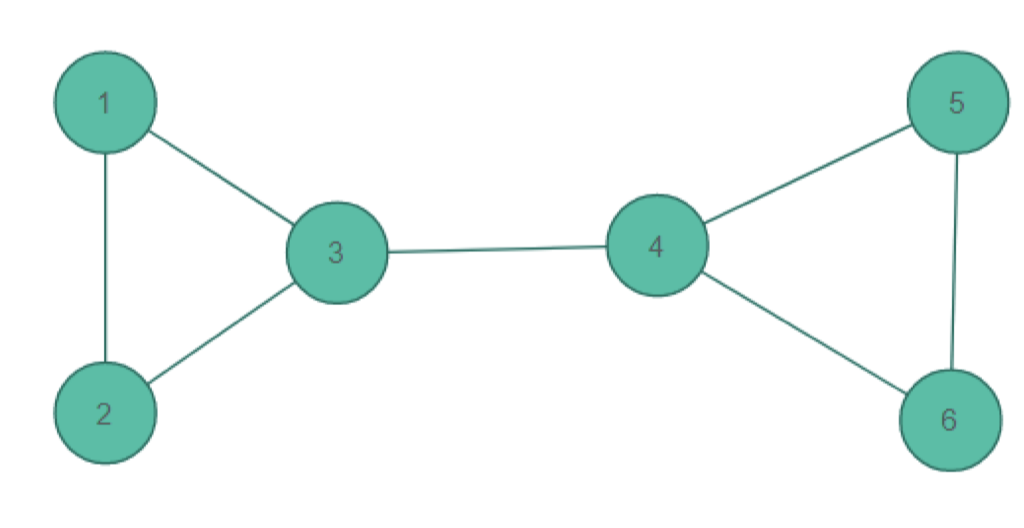
\includegraphics[width=\textwidth]{girvan_1.png}
        \caption{Graph with edge weights based on shortest paths}
        \label{fig:girvan_example}
    \end{figure}
\end{frame}

\begin{frame}[t]{Example of Applying the Girvan–Newman Algorithm}
    \begin{figure}[H]
        \centering
        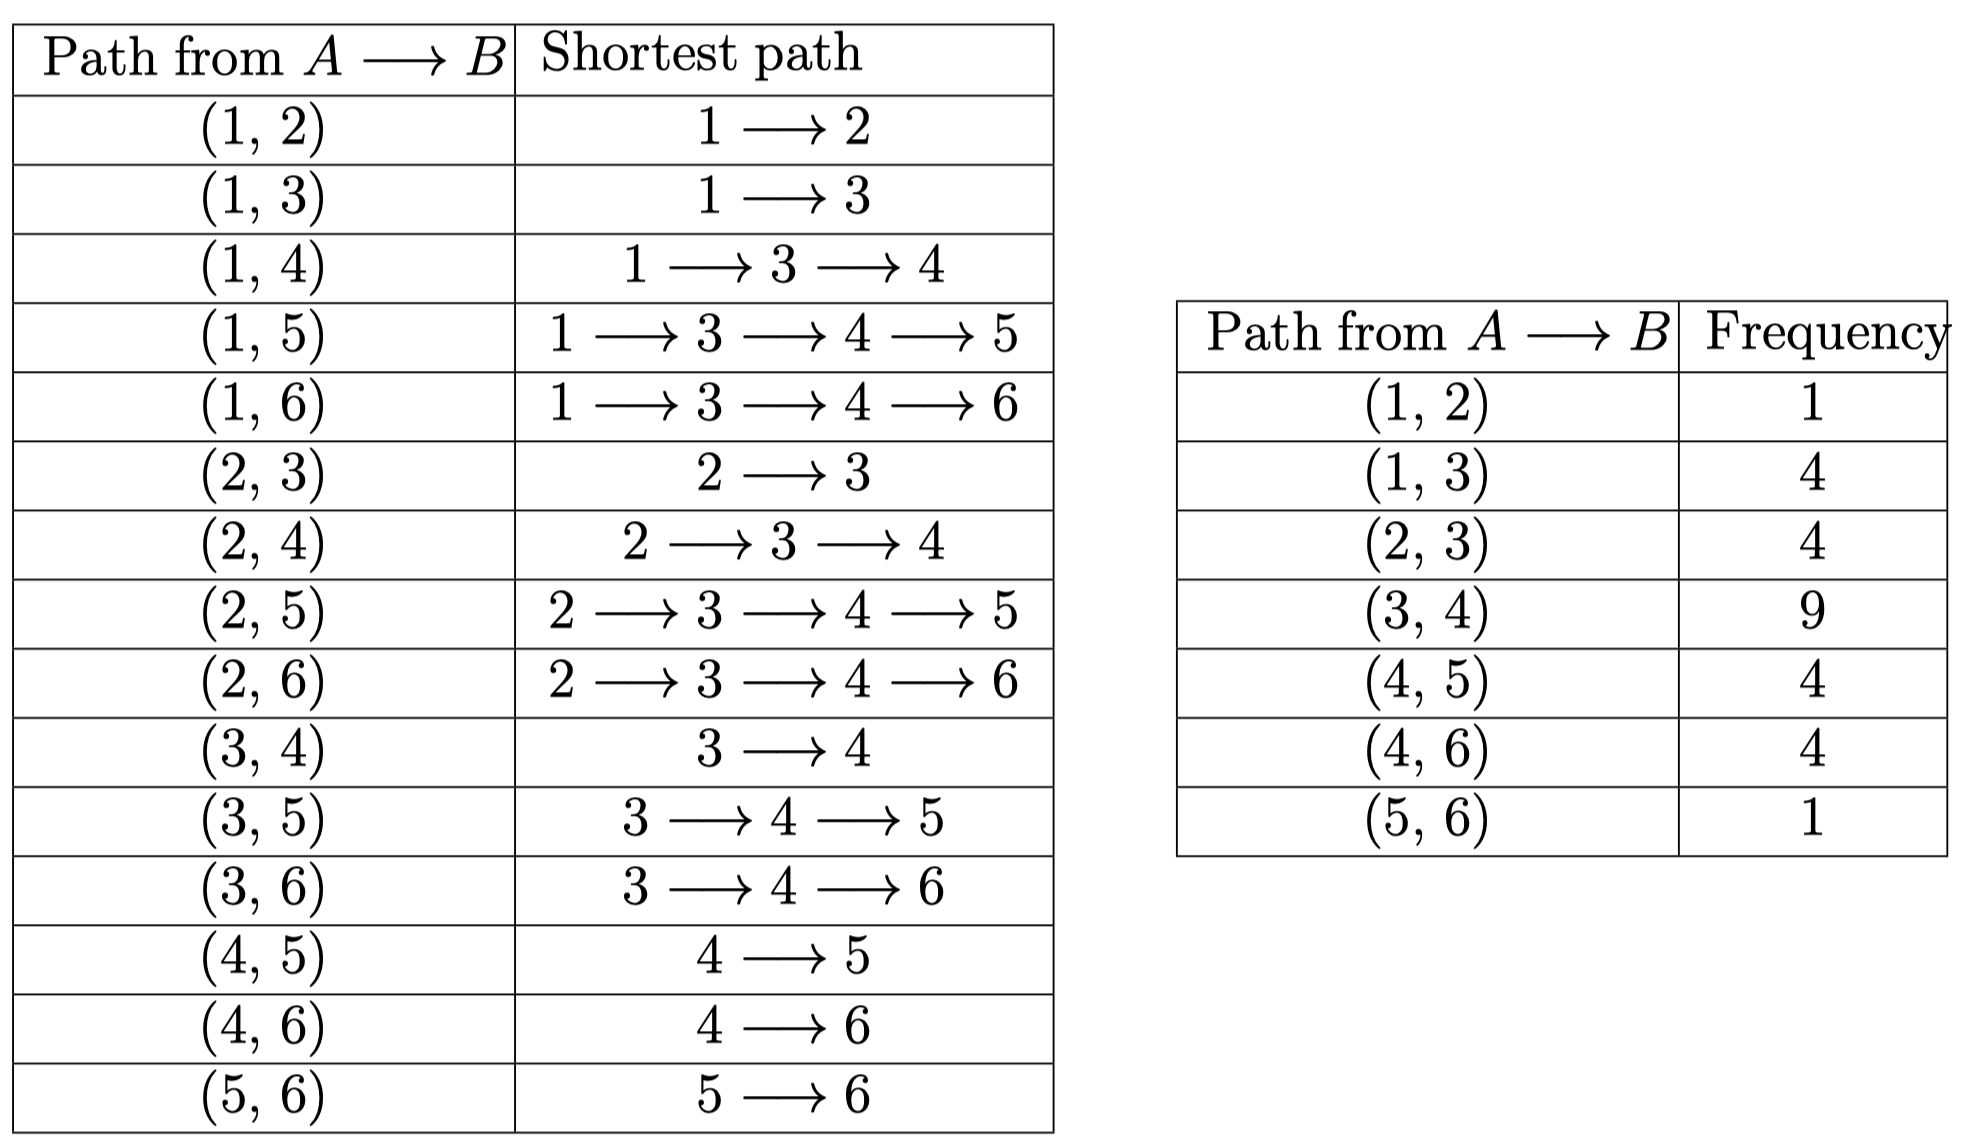
\includegraphics[width=\textwidth]{girvan_2.png}
        \caption{Find the shortest paths and calculate the edge centrality.}
        \label{fig:girvan_example}
    \end{figure}
\end{frame}

\begin{frame}[t]{Example of Applying the Girvan–Newman Algorithm}
    \begin{figure}[H]
        \centering
        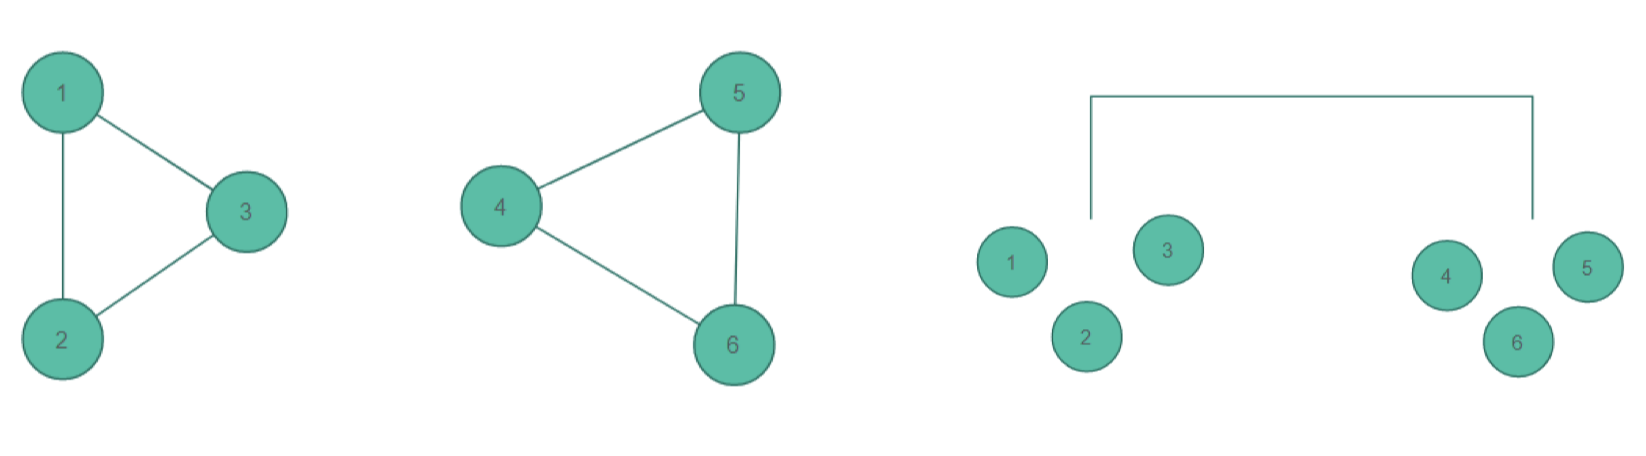
\includegraphics[width=\textwidth]{girvan_3.png}
        \caption{Remove the highest centrality edge and start constructing the dendrogram.}
        \label{fig:girvan_example}
    \end{figure}
\end{frame}

\begin{frame}[t]{Example of Applying the Girvan–Newman Algorithm}
    \begin{figure}[H]
        \centering
        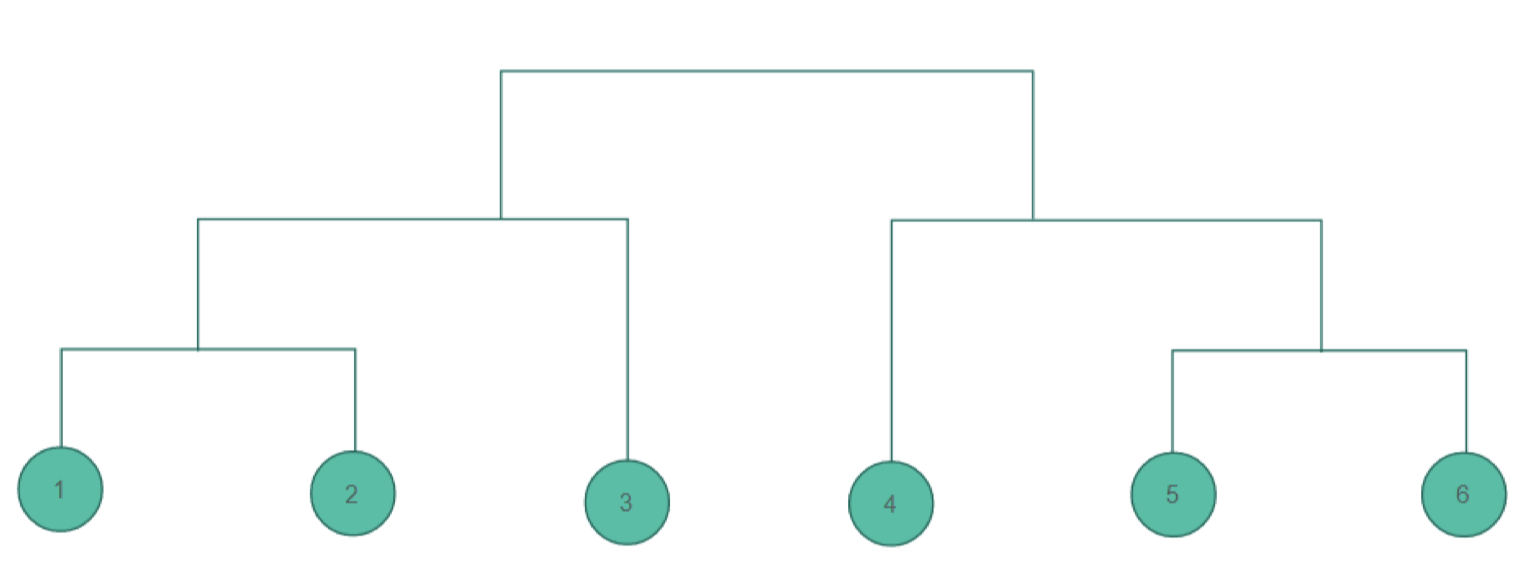
\includegraphics[width=\textwidth]{girvan_result.png}
        \caption{Dendrogram results}
        \label{fig:Dendrogram results}
    \end{figure}
\end{frame}

%Louvain Algorithm
\subsection{Louvain Algorithm}
\begin{frame}[t]{ Louvain Algorithm Overview}
    \textbf{Key Points:}
    \begin{itemize}
        \item  Greedy optimization method aimed at identifying non-overlapping communities within large networks
        \item  Optimizes modularity - a value quantifies the quality of a community structure - using a heuristic approach.
        \item Modularity change when combining 1 node into a community:
\[
\begin{aligned}
    \Delta Q&=Q_c^{updated}-Q_c^{prev}-Q_i^{prev}\\
    &=\left[\frac{\sum in + 2 k_{i,in}}{2m}-\left(\frac{\sum tot+k_i}{2m}\right)^2\right]\\
    &-\left[\frac{\sum in}{2m}-\left(\frac{\sum tot}{2m}\right)^2-\left(\frac{k_i}{2m}\right)^2\right]
\end{aligned}
\]
    \end{itemize}
\end{frame}

\begin{frame}[t]{Louvain Algorithm}
    \small\begin{algorithm}[H]
        \caption{Louvain}\label{alg:louvain}
        \SetKwInOut{Input}{Input}
        \SetKwInOut{Output}{Output}
        \Input{Weighted networks G}
        \Output{Network contains partitioned communities}
        \Repeat{}{
            Put each node of G in its own community\;
            \While{some nodes are moved}{
                \For{all node n of G}{
                place n in its neighboring community including its own which maximizes the modularity gain \;
                }
            }
            \eIf{the new modularity is higher than the initial}{
            G=network between communities of G\;
            }   
            {Terminate\;}
            }
    \end{algorithm}
\end{frame}

% \begin{frame}[t]{Advantages and disadvantages of Louvain}
% \textbf{Advantages}
%   \begin{itemize}
%     \item {Efficiency} 
%     \item {Modularity Optimization}
%     \item {Hierarchical Community Structure} 
%     \item {Flexibility}
%     \item {Robustness}
% \end{itemize}
% \textbf{Disadvantages}
%  \begin{itemize}
%     \item {Resolution Limit}
%     \item {Randomness} 
%     \item {Scalability Issues for Extremely Large Networks} 
%     \item {Lack of Ground Truth Validation}
%     \item {No Overlapping Communities} 
%     \item {Sensitivity to Network Topology}
% \end{itemize}
% \end{frame}

\section{Experiments}
\subsection{Dataset}
\begin{frame}[t]{Dataset}
 \textbf{Summary:}
 \begin{itemize}
 
        \item  "[a] network of books about US politics published around the time of the 2004 presidential election and sold by the online bookseller Amazon.com. Edges between books represent frequent copurchasing of books by the same buyers." 
        \item No weight and no direction
    \end{itemize}
\end{frame}
\begin{frame}[t]{Dataset}
\begin{figure}
    \centering
    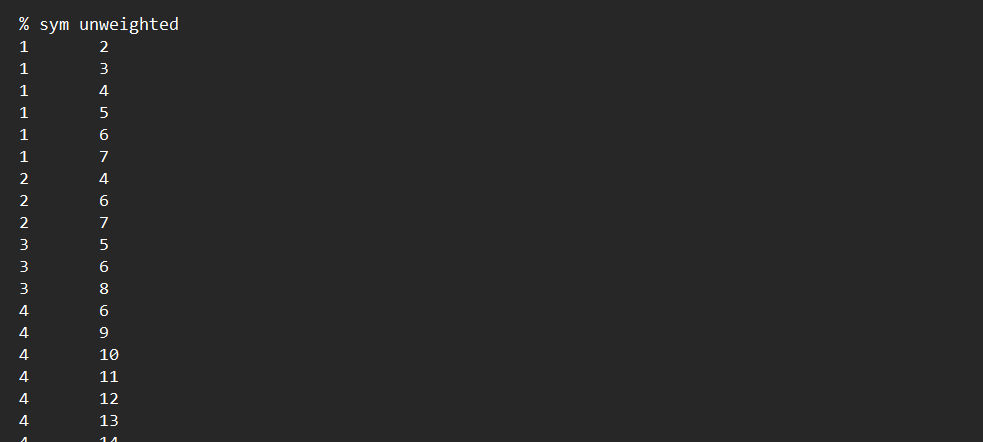
\includegraphics[width=\linewidth]{dataset.png}
\end{figure}
\begin{itemize}
     \item First column: ID of from node.
    \item Second column: ID of to node.
    \end{itemize}
\end{frame}
\subsection{Graph Construction}

\begin{frame}[t]{Graph construction}
 \textbf{Graph construction from TSV file}
 \begin{itemize}
 
        \item Initialize a graph with 105 nodes, where each node represents a political book
        \item Iterate through each of the 441 lines in the input file. If two books are
 frequently co-purchased, an edge is created between their corresponding nodes
    \end{itemize}
\end{frame}
\subsection{Comparative Discussion of Results}
\begin{frame}[t]{Result of hierarchical clustering}
 \begin{itemize}
  \item Optimal Threshold: 10.36
 \item Runtime: 0.000155 seconds
 \item Number of Communities: 2
 \item Community Sizes and Details: 39 nodes and 66 nodes
   \item Most Influential Nodes with Degrees: Node 9, Node 13, Node 4, Node 74, Node 63
 \item Modularity Index: 0.407659
 \end{itemize}
\end{frame}

\begin{frame}[t]{Result of Girvan-Newman algorithm}

 \begin{itemize}
 \item Runtime: 1.1983 seconds
 \item Number of Communities: 2
 \item Community Sizes: 60 nodes and 45 nodes
  \item Most Influential Nodes with Degrees: Node 9, Node 13, Node 4, Node 74, Node 63
 \item Modularity Index: 0.4429
 \end{itemize}
\end{frame}
\begin{frame}[t]{Result of Louvain algorithm}

 \begin{itemize}
 \item Runtime:  0.32 seconds
 \item Number of Communities: 5
 \item Community Sizes and Details: 9 nodes, 33 nodes, 11 nodes, 12 nodes and 40 nodes
   \item Most Influential Nodes with Degrees: Node 9, Node 13, Node 4, Node 74, Node 63
 \item Modularity Index: 0.5268
 \end{itemize}
\end{frame}
\subsection{Discussion}
\begin{frame}[t]{Discussion}
\textbf{Comparative Insights}
\begin{itemize}

  \item Efficiency: Hierarchical Clustering was the fastest, but its results lacked granularity.
 Louvain offered a balance, while Girvan-Newman was the slowest.
 \item Granularity: Louvain identified more communities, indicating a deeper understanding
 of the dataset’s structure. The other methods oversimplified by detecting only two
 groups.
 \item Modularity: Louvain had the highest modularity, making it the most effective at identifying communities with strong internal connections and sparse interconnections
 \end{itemize}
\end{frame}
\subsection{Practical Application}
\begin{frame}[t]{Practical Application: Recommending Books Based on Co-Purchasing Patterns}
With the communities detected using three algorithms, we can apply the results to address the problem of recommending books that are frequently co-purchased and belong to similar communities.

\begin{itemize}
\item \textbf{Input}: A list of book IDs.
\item \textbf{Output}: Determine whether all the books in the list belong to the same community. If not, partition them into clusters of books that are frequently co-purchased.
\end{itemize}

\end{frame}

\begin{frame}[t]{Practical Application: Recommending Books Based on Co-Purchasing Patterns}
Methodology:

\begin{itemize}
    \item Build a graph where:
    \begin{itemize}
        \item Nodes = Books.
        \item Edges = Frequent co-purchasing relationships.
    \end{itemize}
    \item Use three community detection algorithms:
    \begin{itemize}
        \item Hierarchical Clustering
        \item Girvan-Newman Algorithm
        \item Louvain Algorithm
    \end{itemize}
    \item Compare results to recommend books effectively.
    
\end{itemize}

\end{frame}

\begin{frame}[t]{Practical Application: Recommending Books Based on Co-Purchasing Patterns}

For the input:  [2,4,5,7,8], the results based on the communities detected by the three approaches are as follows:
\begin{itemize}
    \item Hierarchical Clustering
    \begin{itemize}
        \item ability\_to\_sell\_together: False
        \item partitions: [[2,5,7,8], [4]]
    \end{itemize}
    \item Girvan-Newman algorithm
    \begin{itemize}
        \item ability\_to\_sell\_together: True
        \item partitions: [[2,4,5,7,8]]
    \end{itemize}
    \item Louvain algorithm
    \begin{itemize}
        \item ability\_to\_sell\_together: False
        \item partitions: [[2,5,7,8], [4]]
    \end{itemize}
\end{itemize}

\end{frame}

\begin{frame}[t]{Practical Application: Recommending Books Based on Co-Purchasing Patterns}

Practical value:
\begin{itemize}
    \item Enhanced Recommendations:
    \begin{itemize}
        \item Suggest books that are likely to be purchased together.
    \end{itemize}
    \item Real-World Impact:
    \begin{itemize}
        \item Personalized shopping experience.
        \item Increased sales through targeted recommendations.
    \end{itemize}
    \item Beyond Books:
    \begin{itemize}
        \item Retail (e.g., groceries, clothing).
        \item Streaming platforms (movies, songs).
    \end{itemize}
\end{itemize}
\end{frame}
\section{Conclusion}
\begin{frame}[t]{Conclusion}
\textbf{US Politics is mainly divided into 2 parties}
\begin{itemize}
  \item Democratic Party (Left-wing)
  \item Republican Party (Right-wing)
 \end{itemize}

 \textbf{Political Spectrum}
\begin{figure}
    \centering
    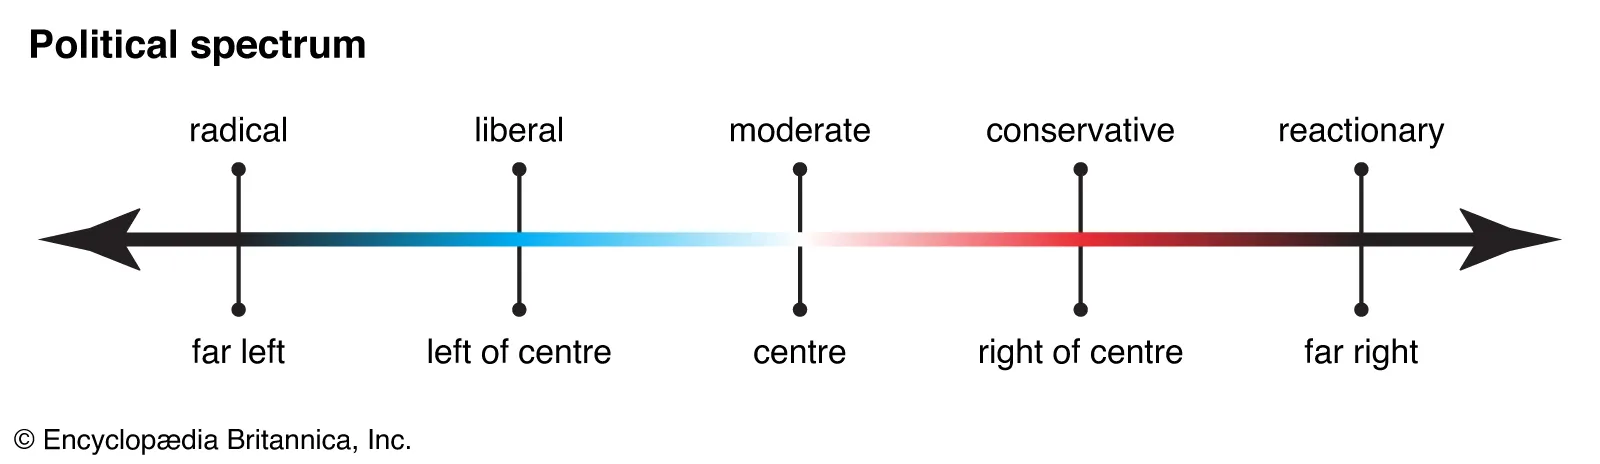
\includegraphics[width=\linewidth]{political_spectrum.png}
\end{figure}
\end{frame}

\begin{frame}[t]{Conclusion}
\textbf{Hierarchical Clustering}
\begin{itemize}
  \item Correctly identified the 2 main wings of US Politics
  \item Is the fastest method
 \end{itemize}

\textbf{Girvan-Newman}
\begin{itemize}
  \item Correctly identified the 2 main wings of US Politics
  \item Slightly better Modularity Index than Hierarchical Clustering
\end{itemize}

\textbf{Louvain}
\begin{itemize}
  \item Correctly identified all 5 communities equivalent to 5 categories of the Political Spectrum
  \item Has the best Modularity Index
  \item Is the median of the 3 in terms of runtime
\end{itemize}
 
\end{frame}
\section{References}

% \begin{frame}[allowframebreaks]{References}
%     \nocite{*}
%     \bibliographystyle{plain}
%     \bibliography{references}
% \end{frame}
\begin{frame}[allowframebreaks]{References}
\begin{thebibliography}{99}

\bibitem[U]{V A Traag et al(2019)}
V. A. Traag et al., 
{\em From Louvain to Leiden: guaranteeing well-connected communities}, 
\url{https://pmc.ncbi.nlm.nih.gov/articles/PMC6435756/}.

\bibitem[U]{Blondel et al(2008)}
Blondel et al., 
{\em Fast Unfolding of Communities in Large Networks}, 
\url{https://www.researchgate.net/publication/1913681_Fast_Unfolding_of_Communities_in_Large_Networks}.

\bibitem[W]{Blondel et al}
Blondel et al., 
{\em Louvain method: Finding communities in large networks}, 
\url{https://sites.google.com/site/findcommunities/}.

\bibitem[G]{Girvan and Newman (2002)}
M. Girvan and M. E. J. Newman, 
{\em Community structure in social and biological networks}, 
Proceedings of the National Academy of Sciences, 99(12), 7821–7826, 
\url{https://www.geeksforgeeks.org/detecting-communities-using-girvan-newman/}.

\bibitem[W]{Ward (1963)}
J. H. Ward Jr., 
{\em Hierarchical Grouping to Optimize an Objective Function}, 
Journal of the American Statistical Association, 58(301), 236–244, 
\url{https://www.tandfonline.com/doi/abs/10.1080/01621459.1963.10500845}.

\bibitem[W]{Poli_spectrum}
{\em Political Spectrum}, 
\url{https://en.wikipedia.org/wiki/Political_spectrum}.

\end{thebibliography}
\end{frame}

\end{document}
